% Auto-generated by tools/paper_online_tikz.py -- lift the tikzpicture into your IEEE paper,
% or compile directly (pdflatex/lualatex). Needs pgfplots >= 1.16. Dense series read .dat tables
% that live next to this file.
\documentclass[tikz,border=2pt]{standalone}
\usepackage{pgfplots}
\pgfplotsset{compat=1.18}
\usepgfplotslibrary{groupplots}
\definecolor{ckv}{RGB}{33,150,243}
\definecolor{cqc}{RGB}{255,152,0}
\definecolor{cql}{RGB}{76,175,80}
\definecolor{cra}{RGB}{244,67,54}
\definecolor{cbanked}{RGB}{46,125,50}
\definecolor{creverted}{RGB}{211,47,47}
\definecolor{cinc}{RGB}{46,125,50}
\definecolor{cret}{RGB}{25,118,210}
\definecolor{coff}{RGB}{211,47,47}
\definecolor{cfrozen}{RGB}{0,0,0}
\begin{document}
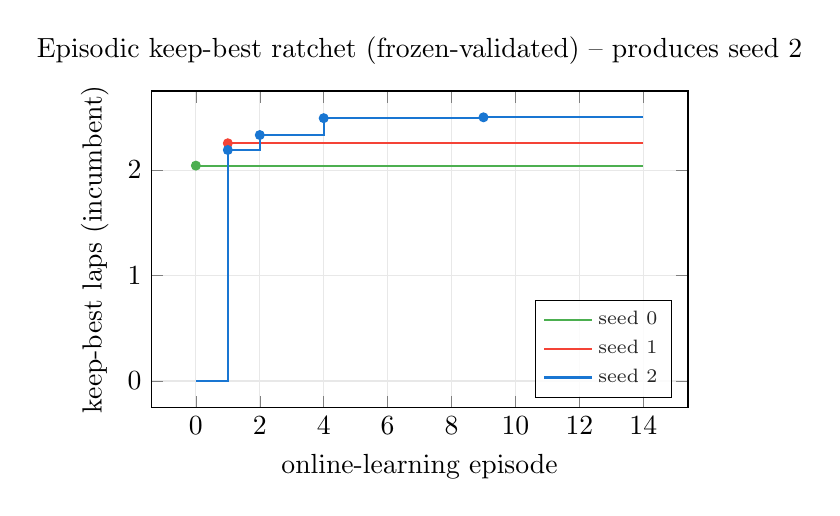
\begin{tikzpicture}
\begin{axis}[width=8.4cm,height=5.6cm,xlabel={online-learning episode},ylabel={keep-best laps (incumbent)},
  title={Episodic keep-best ratchet (frozen-validated) -- produces seed 2},
  grid=both,grid style={gray!18},legend pos=south east,legend style={font=\scriptsize,fill opacity=0.85}]
\addplot[const plot,cql,thick] coordinates {(0,2.042) (1,2.042) (2,2.042) (3,2.042) (4,2.042) (5,2.042) (6,2.042) (7,2.042) (8,2.042) (9,2.042) (10,2.042) (11,2.042) (12,2.042) (13,2.042) (14,2.042)}; \addlegendentry{seed 0}
\addplot[only marks,mark=*,cql,mark size=1.6pt,forget plot] coordinates {(0,2.042)};
\addplot[const plot,cra,thick] coordinates {(0,0) (1,2.254) (2,2.254) (3,2.254) (4,2.254) (5,2.254) (6,2.254) (7,2.254) (8,2.254) (9,2.254) (10,2.254) (11,2.254) (12,2.254) (13,2.254) (14,2.254)}; \addlegendentry{seed 1}
\addplot[only marks,mark=*,cra,mark size=1.6pt,forget plot] coordinates {(1,2.254)};
\addplot[const plot,cret,thick] coordinates {(0,0) (1,2.19) (2,2.332) (3,2.332) (4,2.492) (5,2.492) (6,2.492) (7,2.492) (8,2.492) (9,2.5) (10,2.5) (11,2.5) (12,2.5) (13,2.5) (14,2.5)}; \addlegendentry{seed 2}
\addplot[only marks,mark=*,cret,mark size=1.6pt,forget plot] coordinates {(1,2.19) (2,2.332) (4,2.492) (9,2.5)};
\end{axis}
\end{tikzpicture}
\end{document}
